% Options for packages loaded elsewhere
\PassOptionsToPackage{unicode}{hyperref}
\PassOptionsToPackage{hyphens}{url}
%
\documentclass[
]{article}
\usepackage{amsmath,amssymb}
\usepackage{iftex}
\ifPDFTeX
  \usepackage[T1]{fontenc}
  \usepackage[utf8]{inputenc}
  \usepackage{textcomp} % provide euro and other symbols
\else % if luatex or xetex
  \usepackage{unicode-math} % this also loads fontspec
  \defaultfontfeatures{Scale=MatchLowercase}
  \defaultfontfeatures[\rmfamily]{Ligatures=TeX,Scale=1}
\fi
\usepackage{lmodern}
\ifPDFTeX\else
  % xetex/luatex font selection
\fi
% Use upquote if available, for straight quotes in verbatim environments
\IfFileExists{upquote.sty}{\usepackage{upquote}}{}
\IfFileExists{microtype.sty}{% use microtype if available
  \usepackage[]{microtype}
  \UseMicrotypeSet[protrusion]{basicmath} % disable protrusion for tt fonts
}{}
\makeatletter
\@ifundefined{KOMAClassName}{% if non-KOMA class
  \IfFileExists{parskip.sty}{%
    \usepackage{parskip}
  }{% else
    \setlength{\parindent}{0pt}
    \setlength{\parskip}{6pt plus 2pt minus 1pt}}
}{% if KOMA class
  \KOMAoptions{parskip=half}}
\makeatother
\usepackage{xcolor}
\usepackage[margin=1in]{geometry}
\usepackage{graphicx}
\makeatletter
\def\maxwidth{\ifdim\Gin@nat@width>\linewidth\linewidth\else\Gin@nat@width\fi}
\def\maxheight{\ifdim\Gin@nat@height>\textheight\textheight\else\Gin@nat@height\fi}
\makeatother
% Scale images if necessary, so that they will not overflow the page
% margins by default, and it is still possible to overwrite the defaults
% using explicit options in \includegraphics[width, height, ...]{}
\setkeys{Gin}{width=\maxwidth,height=\maxheight,keepaspectratio}
% Set default figure placement to htbp
\makeatletter
\def\fps@figure{htbp}
\makeatother
\setlength{\emergencystretch}{3em} % prevent overfull lines
\providecommand{\tightlist}{%
  \setlength{\itemsep}{0pt}\setlength{\parskip}{0pt}}
\setcounter{secnumdepth}{-\maxdimen} % remove section numbering
\ifLuaTeX
  \usepackage{selnolig}  % disable illegal ligatures
\fi
\IfFileExists{bookmark.sty}{\usepackage{bookmark}}{\usepackage{hyperref}}
\IfFileExists{xurl.sty}{\usepackage{xurl}}{} % add URL line breaks if available
\urlstyle{same}
\hypersetup{
  pdfauthor={İrfan YAKUT},
  hidelinks,
  pdfcreator={LaTeX via pandoc}}

\author{İrfan YAKUT}
\date{16-11-2023}

\begin{document}

\hypertarget{uxe7oklu-doux11frusal-regresyon-ile-maaux15f-tahmin-modeli}{%
\section{\texorpdfstring{\textbf{Çoklu Doğrusal Regresyon ile Maaş
Tahmin
Modeli}}{Çoklu Doğrusal Regresyon ile Maaş Tahmin Modeli}}\label{uxe7oklu-doux11frusal-regresyon-ile-maaux15f-tahmin-modeli}}

\includegraphics[width=6.36458in,height=\textheight]{https://avatars.mds.yandex.net/i?id=6463706f945bcbf5cc5389be60e023fb3fa08af3-5220968-images-thumbs\&n=13}

Maaş bilgileri ve \textbf{1986} yılına ait kariyer istatistikleri
paylaşılan beyzbol oyuncularının maaş tahminleri için bir doğrusal
regresyon modeli geliştireceğiz.

\textbf{Veri Seti Hikayesi}

Bu veri seti orijinal olarak Carnegie Mellon Üniversitesi'nde bulunan
StatLib kütüphanesinden alınmıştır.

Veri seti 1988 ASA Grafik Bölümü Poster Oturumu'nda kullanılan verilerin
bir parçasıdır.

Maaş verileri orijinal olarak Sports Illustrated, 20 Nisan 1987'den
alınmıştır.

1986 ve kariyer istatistikleri, Collier Books, Macmillan Publishing
Company, New York tarafından yayınlanan 1987 Beyzbol Ansiklopedisi
Güncellemesinden elde edilmiştir.

\textbf{Değişkenler}

\textbf{\emph{20 Değişken 322 Gözlem 21 KB}}

\begin{itemize}
\item
  AtBat 1986-1987 sezonunda bir beyzbol sopası ile topa yapılan vuruş
  sayısı
\item
  Hits 1986-1987 sezonundaki isabet sayısı
\item
  HmRun 1986-1987 sezonundaki en değerli vuruş sayısı
\item
  Runs 1986-1987 sezonunda takımına kazandırdığı sayı
\item
  RBI Bir vurucunun vuruş yaptıgında koşu yaptırdığı oyuncu sayısı
\item
  Walks Karşı oyuncuya yaptırılan hata sayısı
\item
  Years Oyuncunun major liginde oynama süresi (sene)
\item
  CAtBat Oyuncunun kariyeri boyunca topa vurma sayısı
\item
  CHits Oyuncunun kariyeri boyunca yaptığı isabetli vuruş sayısı
\item
  CHmRun Oyucunun kariyeri boyunca yaptığı en değerli sayısı
\item
  CRuns Oyuncunun kariyeri boyunca takımına kazandırdığı sayı
\item
  CRBI Oyuncunun kariyeri boyunca koşu yaptırdırdığı oyuncu sayısı
\item
  CWalks Oyuncun kariyeri boyunca karşı oyuncuya yaptırdığı hata sayısı
\item
  League Oyuncunun sezon sonuna kadar oynadığı ligi gösteren A ve N
  seviyelerine sahip bir faktör
\item
  Division 1986 sonunda oyuncunun oynadığı pozisyonu gösteren E ve W
  seviyelerine sahip bir faktör
\item
  PutOuts Oyun icinde takım arkadaşınla yardımlaşma
\item
  Assits 1986-1987 sezonunda oyuncunun yaptığı asist sayısı
\item
  Errors 1986-1987 sezonundaki oyuncunun hata sayısı
\item
  Salary Oyuncunun 1986-1987 sezonunda aldığı maaş(bin uzerinden)
\item
  NewLeague 1987 sezonunun başında oyuncunun ligini gösteren A ve N
  seviyelerine sahip bir faktör
\end{itemize}

\textbf{Verinin İçeri Aktarılması}

Verimizi ilgili klasörden içeri aktarıyor:

\begin{verbatim}

df <- read.csv("C:\\Users\\GLB90057874\\Desktop\\Denetimli İstatistik\\hitters_eda.csv")
\end{verbatim}

\emph{Veriye ilk bakış:}

\begin{verbatim}

head(df)
\end{verbatim}

\textbf{Çoklu Doğrusal Regresyon Modelinin Tüm Değişkenler ile
Kurulması: Base Model}

Yüksek korelasyona sahip değişkenler hariç diğer değişkenleri ekleyerek
model kuruyoruz.

\begin{verbatim}

base_model=lm(Salary~., data=df)
\end{verbatim}

Özetine ve ilgili katsayılarına bakalım.

\begin{verbatim}

summary(base_model)
\end{verbatim}

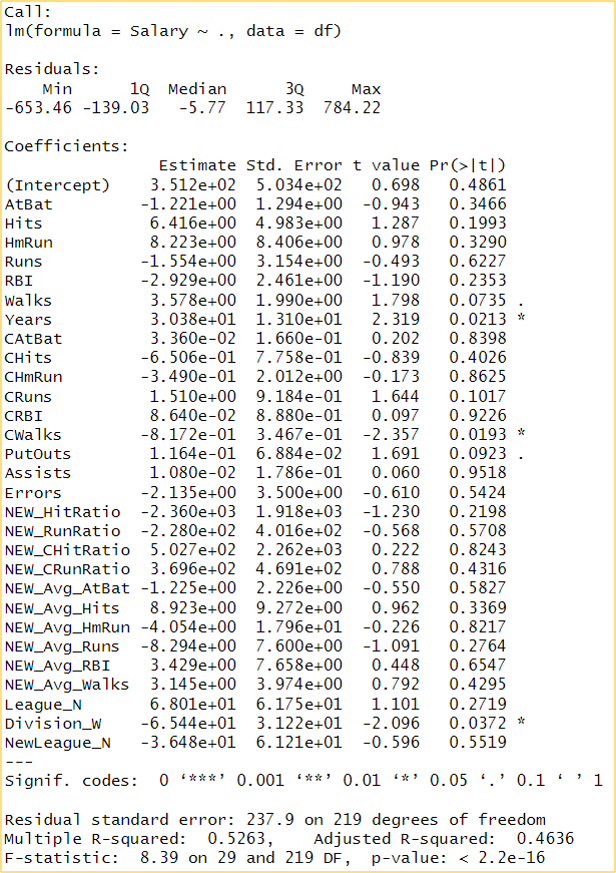
\includegraphics{Picture1.png}

Model istatistiksel olarak anlamlıdır. \textbf{(F-istatistiği = 8.39,
p-değeri \textless{} 2.2e-16).}

R-kare değeri \textbf{0.5263'tür,} bu da modelin Salary değişkenindeki
varyasyonun \textbf{\%52.63}'ünü açıkladığını gösterir. Düzeltilmiş
R-kare değeri \textbf{0.4636}'dır, bu da modeldeki bağımsız
değişkenlerin sayısını dikkate alır.

Modeldeki en önemli değişkenler \textbf{Years , NEW\_HitRatio ve
CWalks}'tır. Artıklar yaklaşık olarak normal dağılmıştır.

Genel olarak, base\_model verilere iyi bir uyum sağlar ve Salary
değişkenindeki varyasyonun önemli bir kısmını açıklar. Modeldeki en
önemli bağımsız değişkenler ise \textbf{Years, NEW\_HitRatio ve
CWalks'}tır.

\emph{VIF değerlerini inceleyelim:}

\begin{verbatim}

library(car)
vif(base_model) #VIF değerlerini yazdırır.
\end{verbatim}

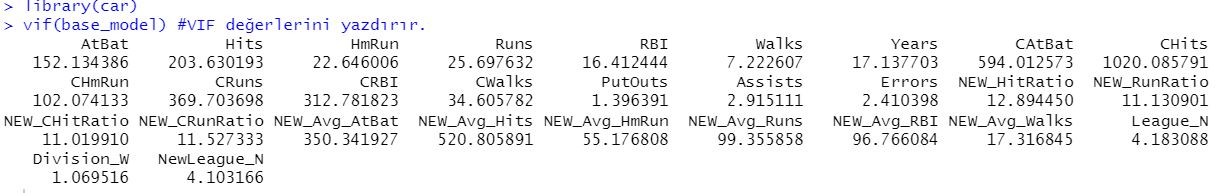
\includegraphics[width=7.20833in,height=\textheight]{Capture.JPG}

\textbf{\emph{Yüksek VIF (10'dan büyük):}}

AtBat, Hits, CAtBat, CHits, NEW\_Avg\_AtBat, NEW\_Avg\_Hits: Bu
değişkenlerin VIF değerleri nispeten yüksek, bu da bu değişkenler
arasında potansiyel çoklu doğrusallık sorunları olduğunu gösteriyor. Bu,
bu değişkenlerin birbirleriyle ilişkili olabileceği anlamına gelir ve
bağımlı değişken üzerindeki etkilerini izole etmeyi zorlaştırabilir.

\textbf{\emph{Orta Seviye VIF (5 ile 10 arası):}}

HmRun, Runs, RBI, Years, CHmRun, CRuns, CRBI, CWalks, PutOuts, Assists,
NEW\_HitRatio, NEW\_RunRatio, NEW\_CHitRatio, NEW\_CRunRatio,
NEW\_Avg\_HmRun, NEW\_Avg\_Runs, NEW\_Avg\_RBI, NEW\_Avg\_Walks: Bu
değişkenlerin VIF değerleri orta seviyede. Tek başlarına sorunlu
olmayabilirler, ancak diğer değişkenlerle birlikte etkileşimleri çoklu
doğrusallığa neden olabilir.

\textbf{\emph{Düşük VIF (5'ten küçük):}}

Walks, Errors, League\_N, Division\_W, NewLeague\_N: Bu değişkenlerin
VIF değerleri nispeten düşük, bu da onların çoklu doğrusallıktan daha az
etkilendiğini gösteriyor.

\textbf{WIF Değerlerine Göre Base\_Model2'nin Kurulması}

Çoklu doğrusallıktan etkilenmemek adına ve daha iyi bir performans
modeli için farklı bir model kuruyoruz.

Bu modelde WIF değerleri baz alınarak yeni üretilen değişkenler
üzerinden kuracağız.

\begin{verbatim}

base_model2=lm(Salary~Walks+PutOuts+Assists+Errors+NEW_HitRatio+NEW_RunRatio+NEW_CHitRatio+NEW_CRunRatio+League_N+Division_W+NewLeague_N, data=df)

summary(base_model2)

vif(base_model2)
\end{verbatim}

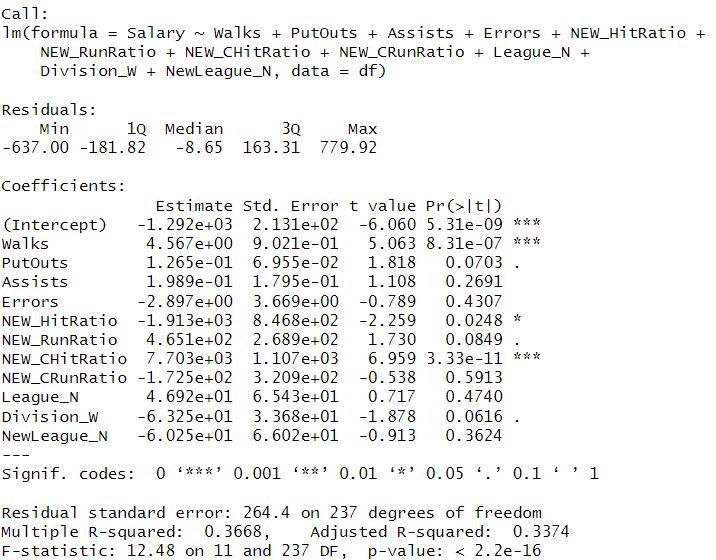
\includegraphics{Capture2.JPG}

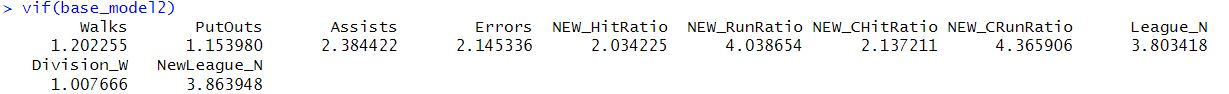
\includegraphics[width=10.46875in,height=\textheight]{Capture3.JPG}\textbf{Değişken
Seçim Yöntemlerinin Kullanılması ve Model Değerlendirme}

\begin{verbatim}

library(olsrr)
library("ISLR")
library(car)

a=ols_step_all_possible(base_model2)
plot(a)
summary(a)
\end{verbatim}

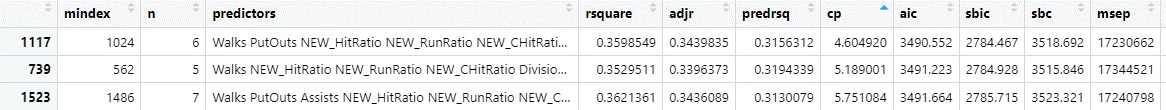
\includegraphics[width=9.83333in,height=\textheight]{Picture2.png}

Cp değerlerine göre \textbf{1024} nolo modelde \textbf{Walks PutOuts
NEW\_HitRatio NEW\_RunRatio NEW\_CHitRatio Division\_W N:6 CP:4.60}
olarak çıkmıştır ve modeli en iyi açıklayan baz değişkenlerin bu şekilde
olduğunu söyleyebiliriz.

\begin{verbatim}

s=ols_step_both_p(base_model2)
s=ols_step_both_p(base_model2, pent = 0.05, prem = 0.1)
s
s$base_model2
plot(s)
\end{verbatim}

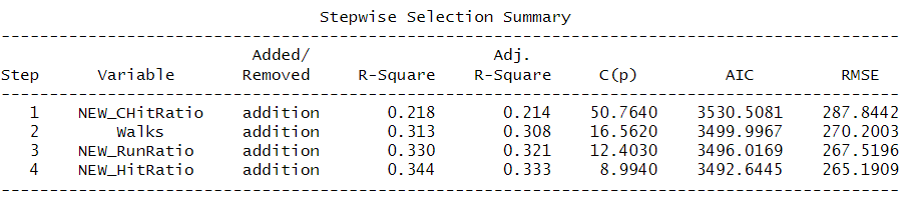
\includegraphics{Picture3.png}Stepwise yöntemi ile de seçim yaptığımızda
R2 ve Düzeltimiş R2 değerleri özellikle 4 değişken içerisinde artış
gösterdiğini görüyoruz.

\textbf{Base\_Model3 Oluşturulması ve Matrix Plot Çizimi}

\begin{verbatim}

base_model3=lm(Salary~Walks+PutOuts+NEW_HitRatio+NEW_RunRatio+NEW_CHitRatio+Division_W, data=df)
summary(base_model3)
\end{verbatim}

Base\_model3 özetine baktığımızda R2'nin düşüş gösterdiğini görüyoruz.

\begin{verbatim}

base_model3df <- data.frame(df$Walks, df$Salary, df$PutOuts,df$NEW_HitRatio,df$NEW_RunRatio,df$NEW_CHitRatio,df$Division_W)
pairs(base_model3df, pch=19, col='red', lower.panel = NULL)
\end{verbatim}

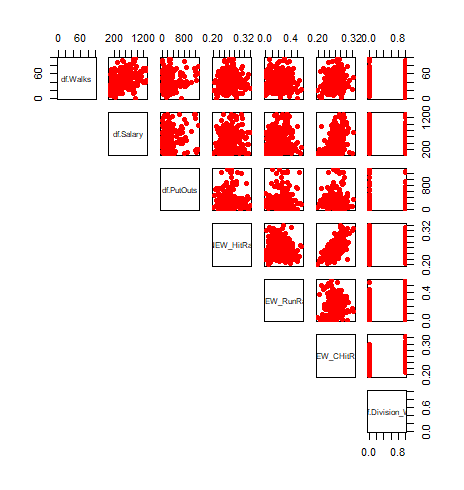
\includegraphics[width=6.89583in,height=\textheight]{Rplot.png}

\textbf{Değişkenlerin Normalleştirilmesi için Dağılım Grafiklerinin
Kontrolü}

\begin{verbatim}

y_variable <- df$Walks
hist(my_variable, col = "skyblue", main = "Değişkenin Dağılımı", xlab = "Değerler", ylab = "Frekans") #log alacağız

my_variable <- df$PutOuts
hist(my_variable, col = "skyblue", main = "Değişkenin Dağılımı", xlab = "Değerler", ylab = "Frekans") #log alacağız

my_variable <- df$NEW_HitRatio
hist(my_variable, col = "skyblue", main = "Değişkenin Dağılımı", xlab = "Değerler", ylab = "Frekans") #log alacağız

my_variable <- df$NEW_RunRatio
hist(my_variable, col = "skyblue", main = "Değişkenin Dağılımı", xlab = "Değerler", ylab = "Frekans") #log alacağız

my_variable <- df$NEW_CHitRatio
hist(my_variable, col = "skyblue", main = "Değişkenin Dağılımı", xlab = "Değerler", ylab = "Frekans") #log alacağız
\end{verbatim}

Değişkenler üzerinde istatiksel işlemler yapmadan önce dağılım
grafiklerinin kontrolünü sağlıyoruz. Sayısal değişkenler üzerinde log
dönüşümü yaparak modeli tekrar oluşturuyoruz.

\begin{verbatim}

log_transform_vars <- c("Walks", "PutOuts", "NEW_HitRatio", "NEW_RunRatio", "NEW_CHitRatio")
df[log_transform_vars] <- log(df[log_transform_vars] + 1)  # +1 eklenmesi log(0) hatasını önler

log_transform_model <- lm(Salary ~ Walks + PutOuts + NEW_HitRatio + NEW_RunRatio + NEW_CHitRatio + Division_W, data = df)

summary(log_transform_model)
\end{verbatim}

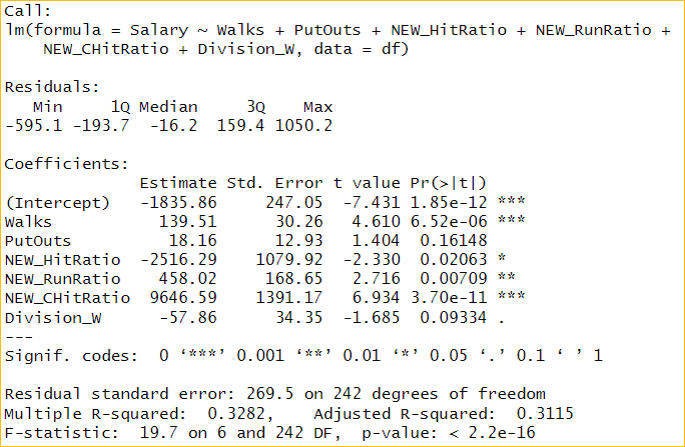
\includegraphics{Picture5.png}\textbf{Log Alınmış Model Matrix Plot
Çizimi}

\begin{verbatim}

log_transform_modeldf <- data.frame(df$Walks, df$Salary, df$PutOuts,df$NEW_HitRatio,df$NEW_RunRatio,df$NEW_CHitRatio,df$Division_W)
pairs(log_transform_modeldf, pch=19, col='red', lower.panel = NULL)
\end{verbatim}

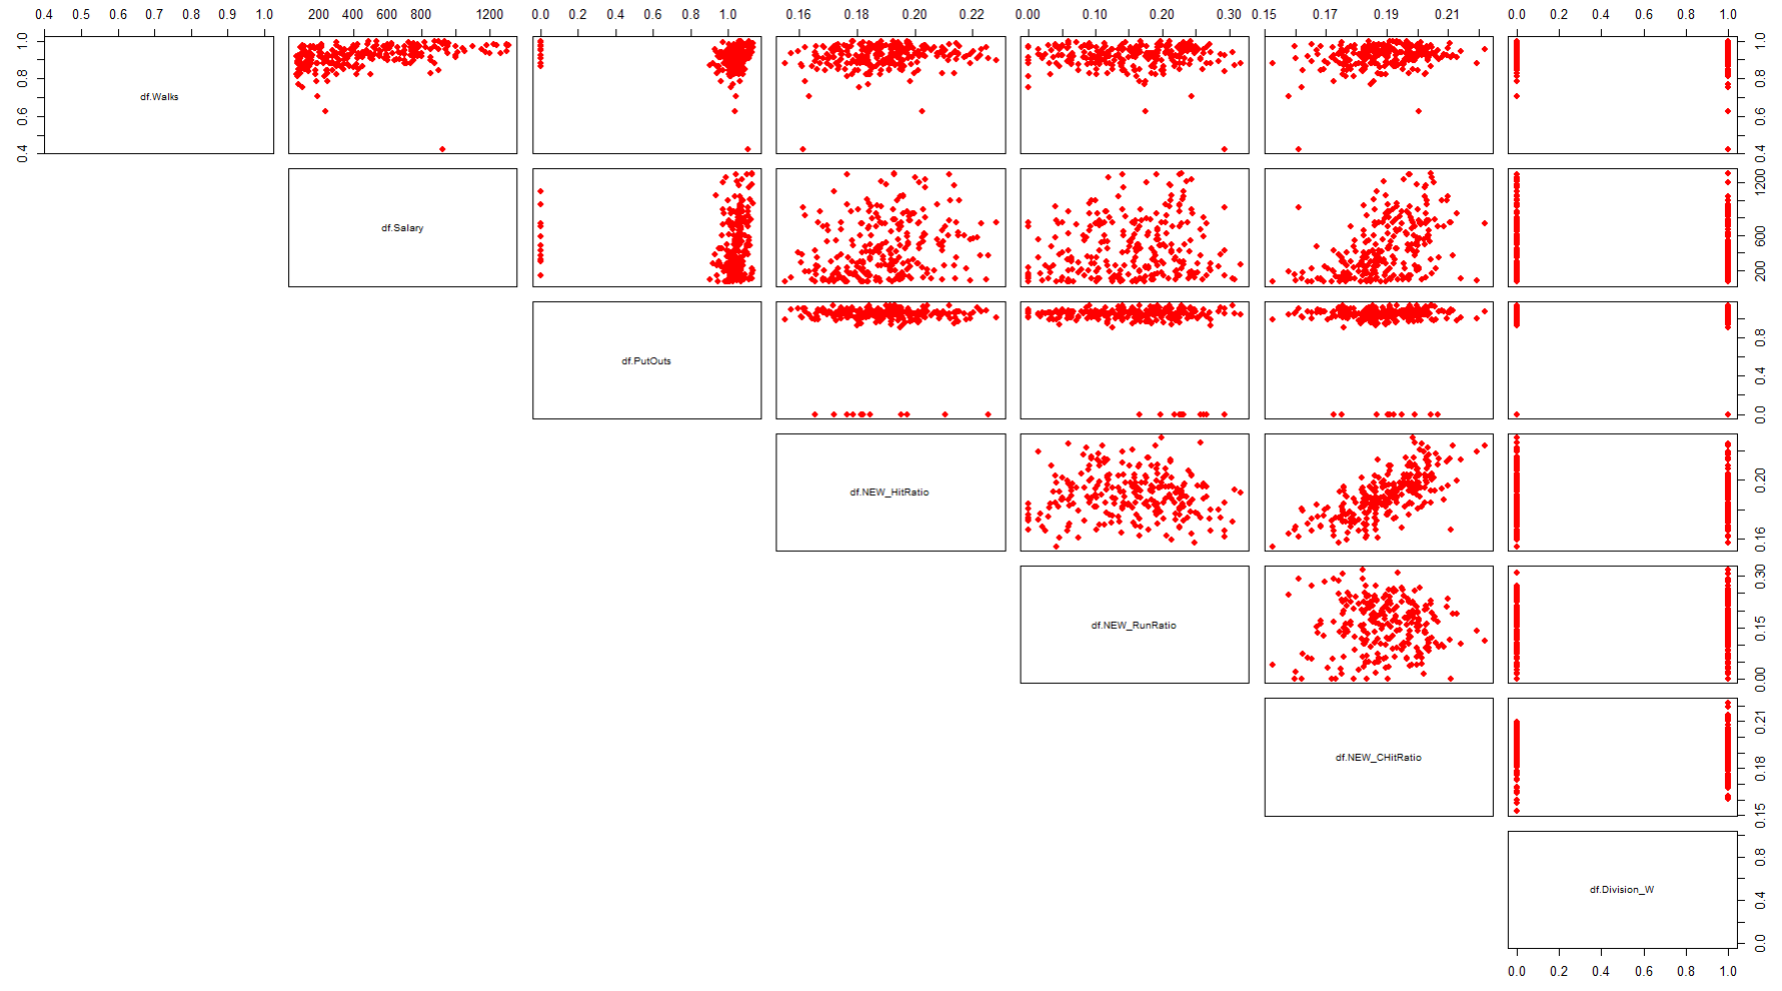
\includegraphics{Picture7.png}\textbf{Hataların Normal Dağıldığını
Kontrol Etme}

\begin{verbatim}

qqnorm(log_transform_model$residuals)
qqline(log_transform_model$residuals)
\end{verbatim}

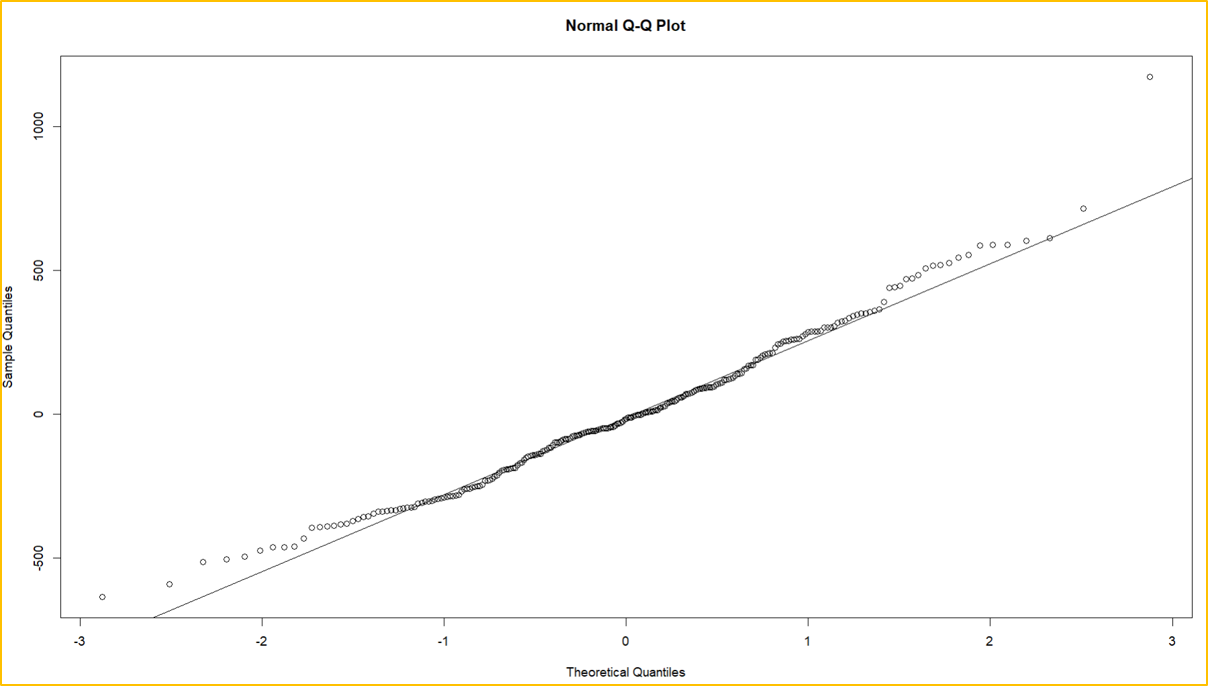
\includegraphics{Picture8.png}\textbf{Kolmogorov-Smirnov Testi}

\begin{verbatim}

ks.test(log_transform_model$residuals, "pnorm")
\end{verbatim}

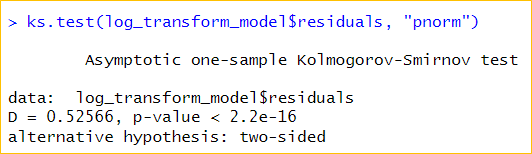
\includegraphics[width=7.15625in,height=\textheight]{Picture9.png}

Bu test sonuçlarına göre, regresyon modelinizin hata terimleri normal
bir dağılıma uymamaktadır. p değeri çok düşük olduğu için, null hipotez
(veri setinin normal bir dağılıma sahip olduğu) reddedilir. Bu durumda,
modelinizin normalite varsayımı karşılamadığını söyleyebiliriz.

\textbf{Hataların Sabit Varyanslı Olup Olmadığını Kontrolü}

Hataların standartlaştırılmış (Studentized) değerlerini elde etmek için

\begin{verbatim}

log_transform_model_stand_residuals <- rstandard(log_transform_model)
\end{verbatim}

Hataların standartlaştırılmış değerlerini görselleştirmek için

\begin{verbatim}

plot(log_transform_model_stand_residuals, ylab = "Standartlaştırılmış Hatalar", xlab = "Gözlemler")
abline(h = 0, col = "red", lty = 2)
\end{verbatim}

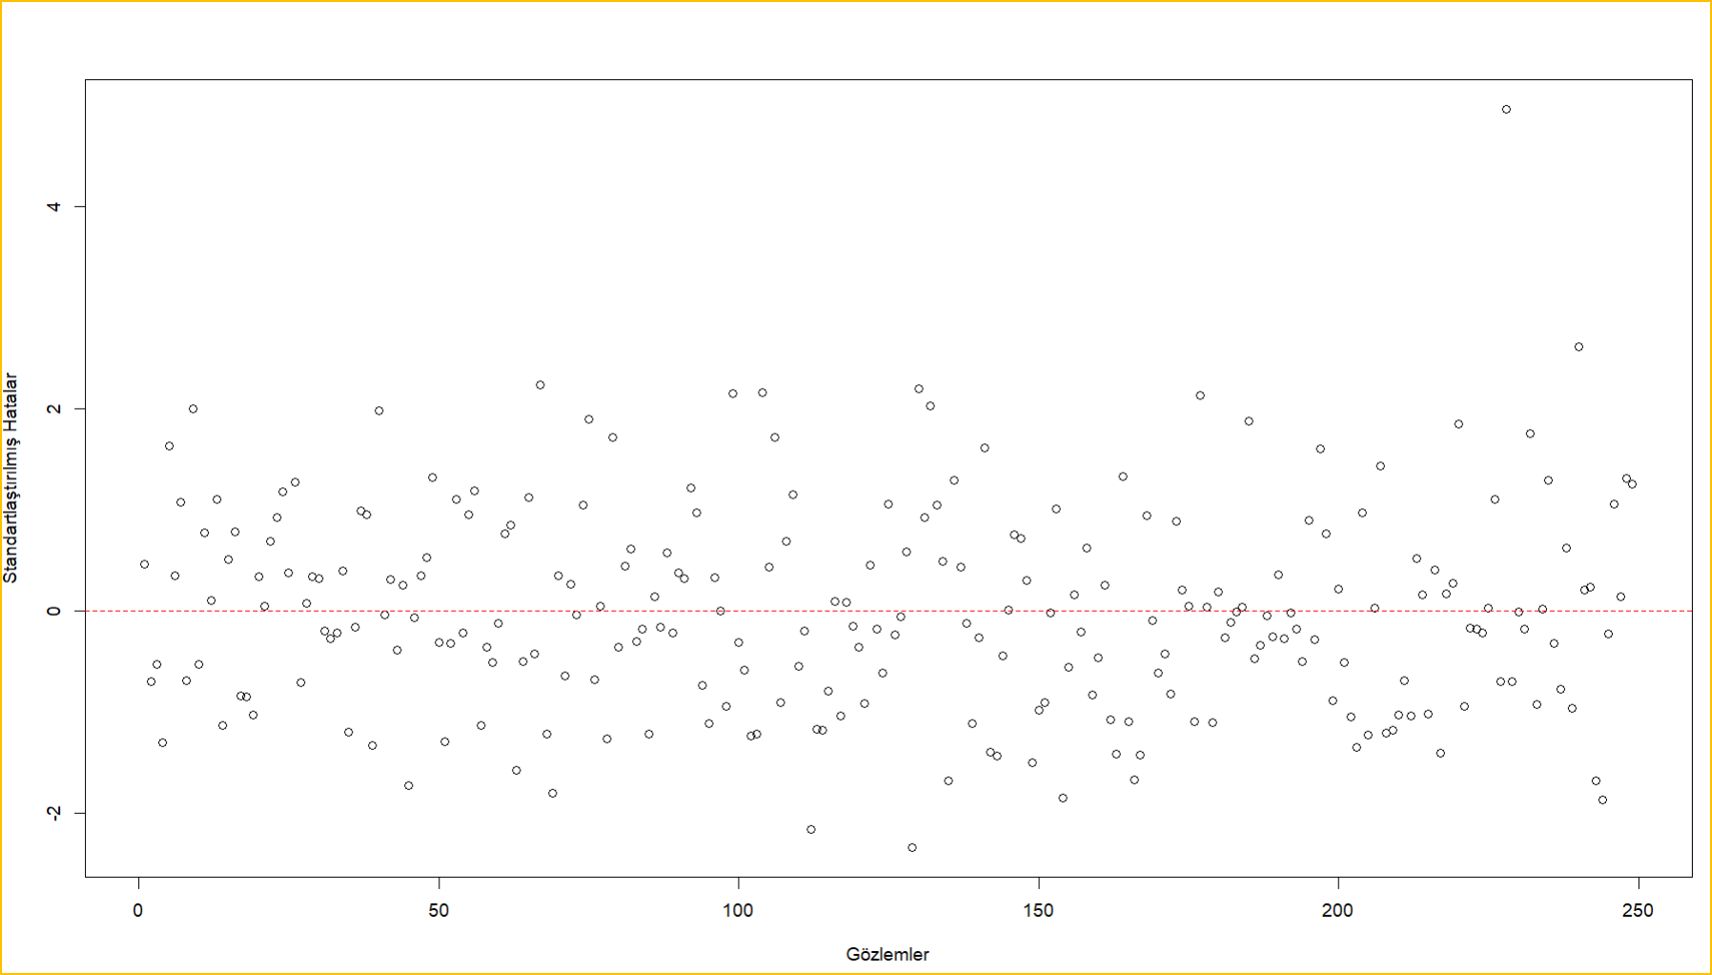
\includegraphics{Picture10.png}Residual plot çizimi

\begin{verbatim}

plot(log_transform_model, which = 1)
\end{verbatim}

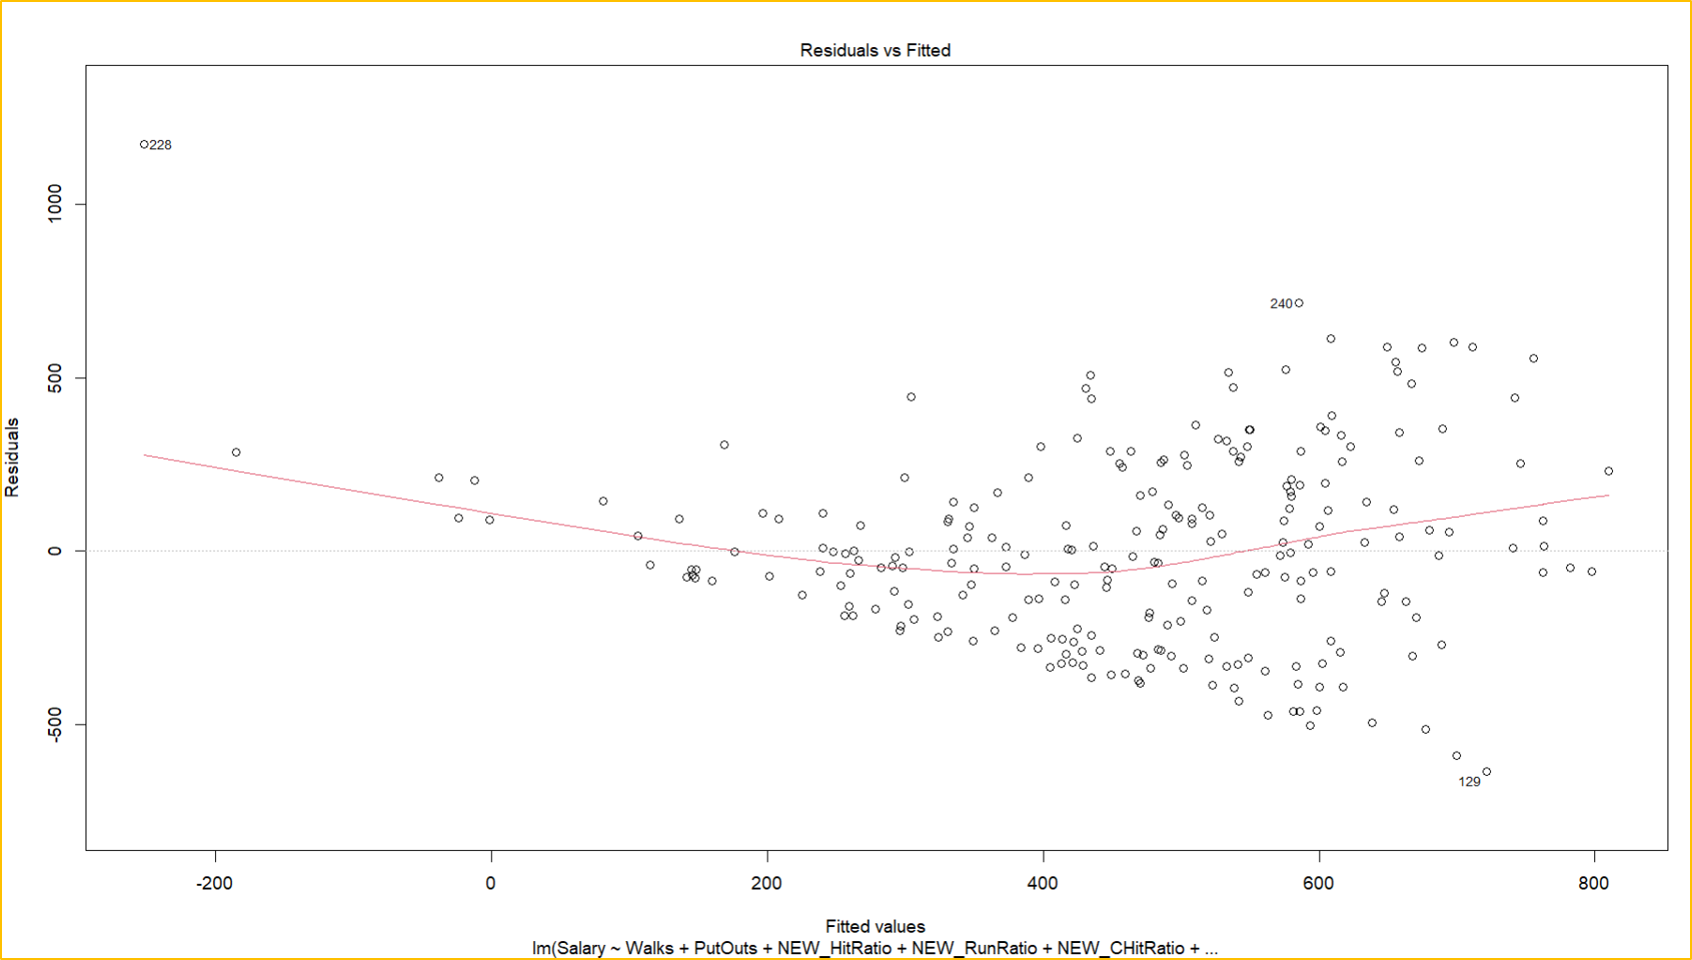
\includegraphics{Picture11.png}\textbf{Uç Değer ve Etkin Gözlem
Kontrolü}

Cook's Distance hesaplanması:

\begin{verbatim}

cooksd <- cooks.distance(log_transform_model)
\end{verbatim}

Cook's Distance grafikle görselleştirme

\begin{verbatim}

plot(cooksd, pch = "o", cex = 1, main = "Cook's Distance")
abline(h = 4/length(log_transform_model$residuals), col = "red", lty = 2)
\end{verbatim}

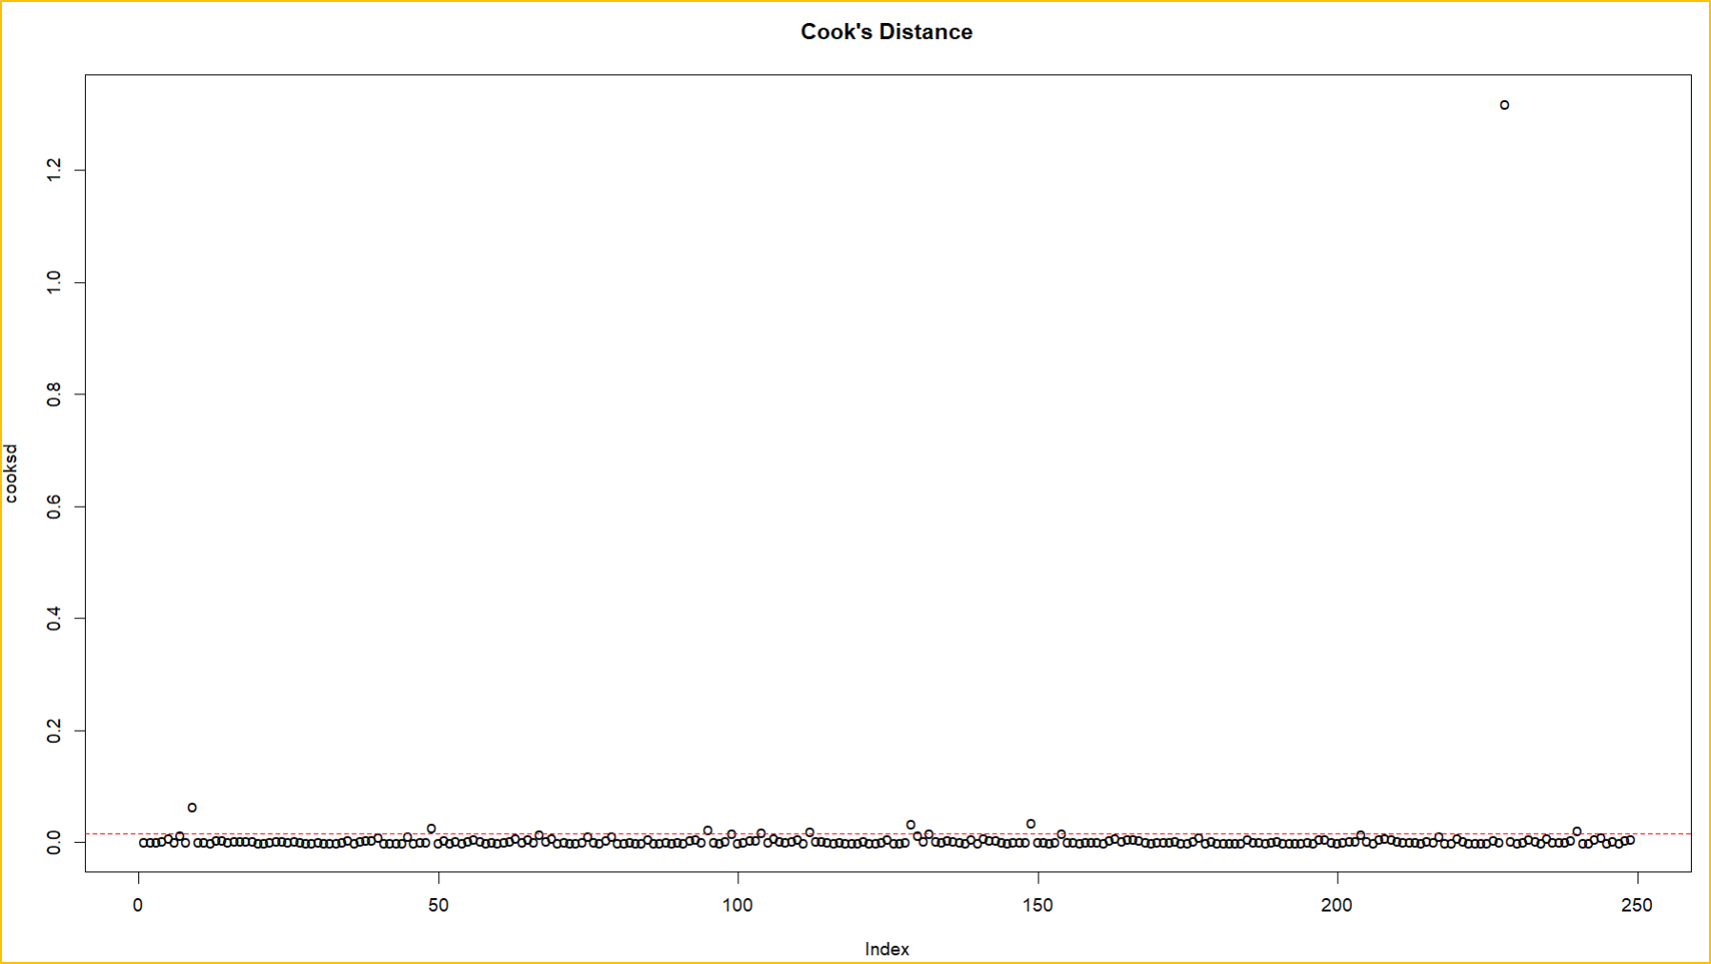
\includegraphics{Picture12.png}Residuals vs.~Leverage grafik

\begin{verbatim}

par(mfrow = c(1, 1))
plot(log_transform_model, which = 5)
\end{verbatim}

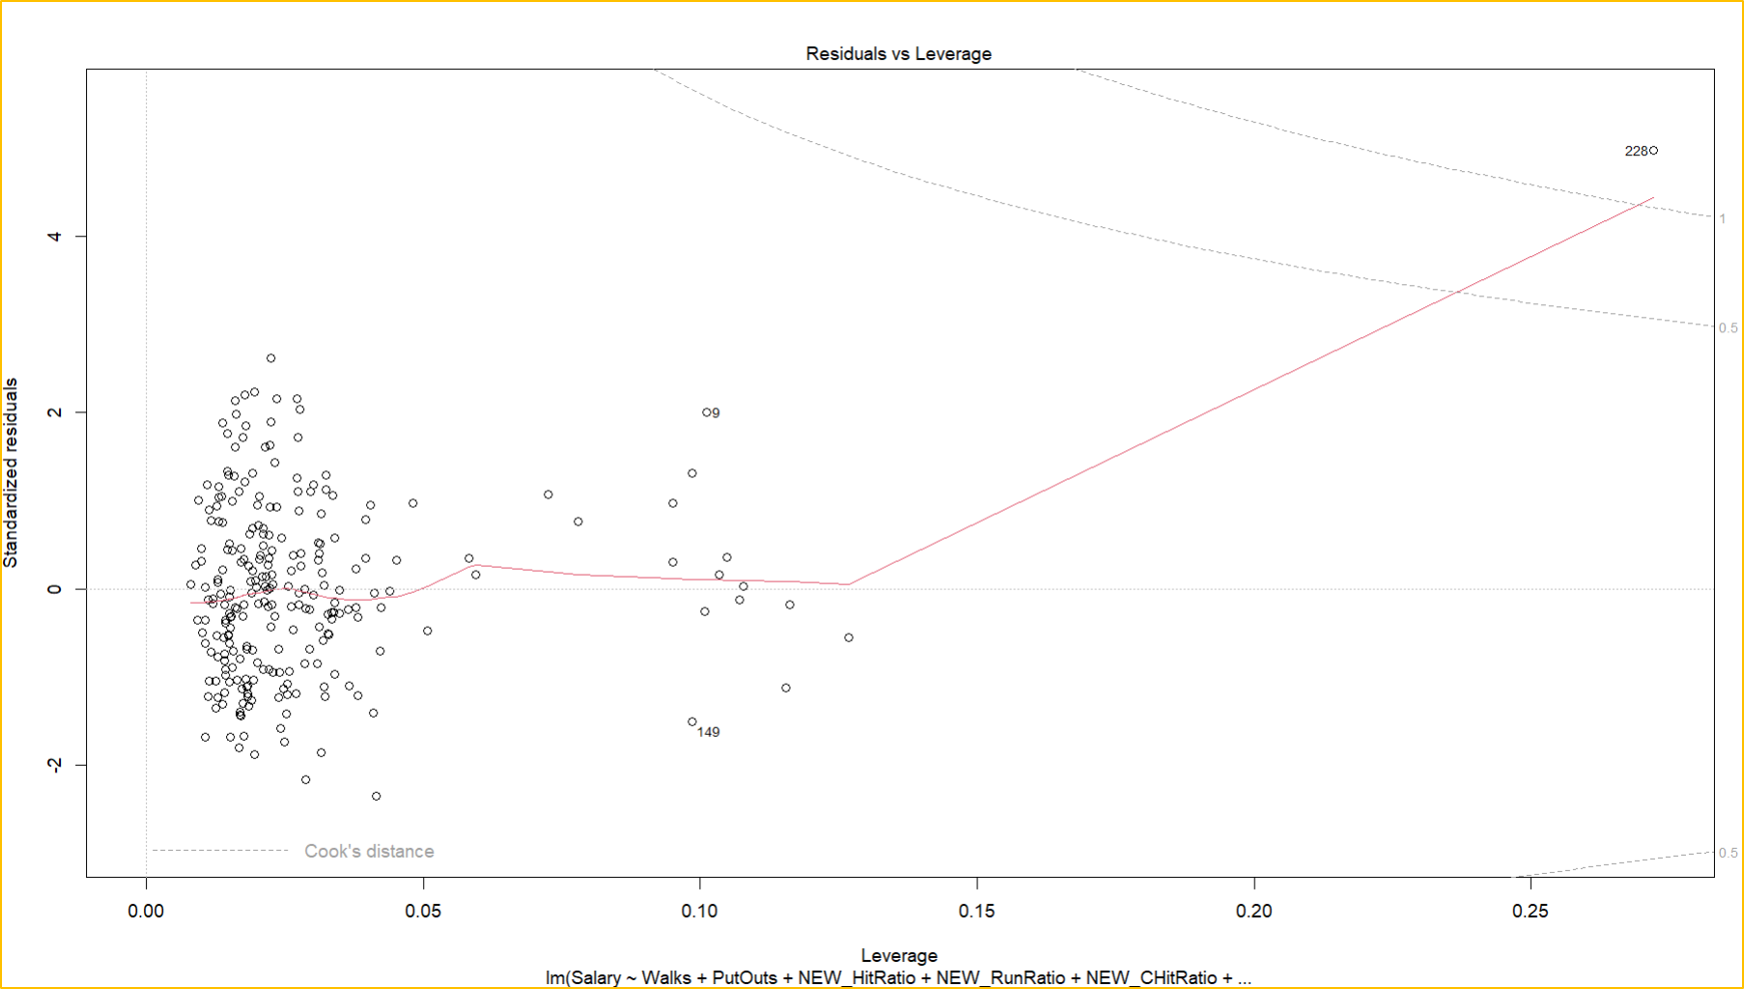
\includegraphics{Picture13.png}\textbf{VIF Değer Kontrolü}

\begin{verbatim}

vif(log_transform_model)
\end{verbatim}

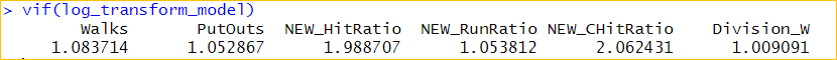
\includegraphics{Picture6.png}\textbf{Final Model Katsayıları}

\begin{verbatim}

summary(log_transform_model)
\end{verbatim}

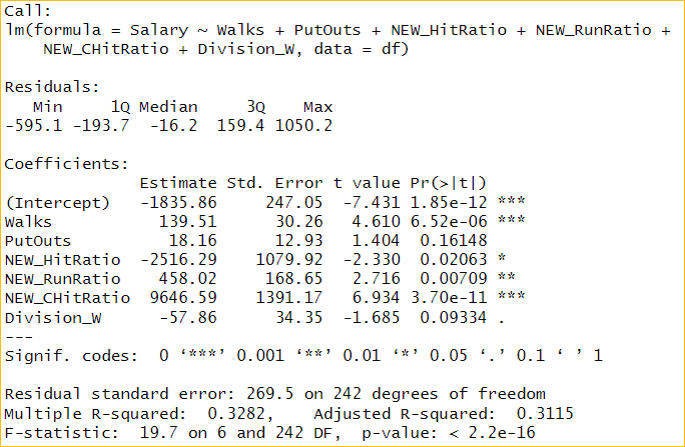
\includegraphics{Picture5.png}\textbf{Katsayıların \%95'lik Güven
Aralıklarını Elde Etmek}

Güven ve Tahmin Aralıkları

\begin{verbatim}

confint(log_transform_model)
confint(log_transform_model,level=0.95)
\end{verbatim}

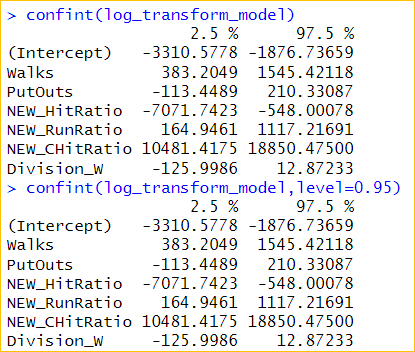
\includegraphics{Picture14.png}

\textbf{Yeni Bir Gözlem Değeri için \%95'lik Güven Aralığını ve Kestirim
Aralığını Oluşturma}

Walks + PutOuts + NEW\_HitRatio + NEW\_RunRatio + NEW\_CHitRatio +
Division\_W

\emph{Yeni gözlem değeri için 95\% güven aralığı}

\begin{verbatim}

new_observation <- data.frame(Walks = 0.99, 
                              PutOuts = 1.11, 
                              NEW_HitRatio = 0.20, 
                              NEW_RunRatio = 0.29, 
                              NEW_CHitRatio = 0.20, 
                              Division_W = 1)
predict_interval <- predict(log_transform_model, newdata = new_observation, interval = "confidence", level = 0.95)
\end{verbatim}

\begin{verbatim}

cat("95% Güven Aralığı:", predict_interval[1], "ile", predict_interval[2], "\n")
\end{verbatim}

\textbf{95\% Güven Aralığı: 715.3476 ile 615.5252}

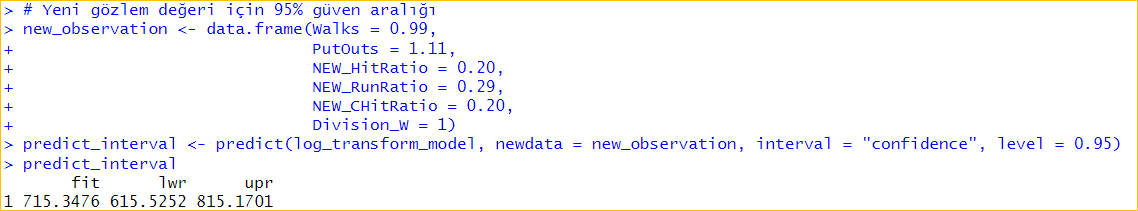
\includegraphics{Picture15.png}

\emph{Yeni gözlem değeri için tahmin ve 95\% kestirim aralığı}

\begin{verbatim}

predict_interval <- predict(log_transform_model, newdata = new_observation, interval = "prediction", level = 0.95)
\end{verbatim}

\begin{verbatim}

cat("95% Kestirim Aralığı:", predict_interval[1], "ile", predict_interval[2], "\n")
\end{verbatim}

\textbf{95\% Kestirim Aralığı: 715.3476 ile 161.6556}

\textbf{Model'i Geliştirmek Üzere Görüş ve Öneriler}

\begin{itemize}
\item
  Modeldeki yeni türetilen ve mevcut değişkenler gözden geçirebilir,
  analize düşük, korelasyonu yüksek değişkenler çıkarılabilir.
\item
  Değişkenlere uygulanan dönüşümleri gözden geçirebiliriz. Belki de
  farklı dönüşümler veya ölçeklemeler kullanarak modelin performansını
  artırabiliriz.
\item
  Bağımsız değişkenler arasındaki çoklu doğrusallığı kontrol ettikten
  sonra bu değişkenlerde dönüşümler ya da farklı ölçeklemeler ile
  kontrol sağlayabiliriz.
\item
  Veri setini genişletmeli, mümkünse daha çok gözlem değeri elde
  etmeliyiz.
\item
  Tüm değişkenler ile kurulan modelden sonrasında değişken seçimi
  yapmalı ve sonrasında değişimler ve dönüşümler uygulamalıyız.
\end{itemize}

\end{document}
